\chapter{Market Analysis}

\section{Industry Overview}

\subsection{Business Networking Platforms}
The premium business networking market has experienced significant growth, driven by:
\begin{itemize}
    \item Increasing demand for exclusive networking opportunities
    \item Rise of high-net-worth individuals seeking peer connections
    \item Digital transformation of traditional networking models
    \item Growing importance of deal flow and investment opportunities
\end{itemize}

\subsection{Market Size and Growth}
\begin{itemize}
    \item Global business networking market: \$XX billion (2024)
    \item DACH region premium networking: \$XX million
    \item Expected CAGR: X\% (2024-2029)
    \item Target addressable market: 50,000+ potential members
\end{itemize}

\section{Business Warfare Strategy: The Art of Competitive Dominance}

\subsection{Strategic Framework: 兵者诡道也 (War is the Way of Deception)}

The BCD platform adopts a sophisticated business warfare strategy inspired by Sun Tzu's Art of War, recognizing that "all warfare is based on deception." This approach encompasses psychological operations, cyber warfare, human resource battles, and public relations campaigns to achieve competitive dominance in the premium networking market.

\subsection{Competitive Battlefield Analysis}

\subsubsection{Primary Adversaries}
\begin{itemize}
    \item \textbf{YPO (Young Presidents' Organization)}: The Goliath - Global leadership network with 30,000+ members, representing the most formidable opponent
    \item \textbf{EO (Entrepreneurs' Organization)}: The Agile Challenger - Peer-to-peer learning network with rapid expansion capabilities
    \item \textbf{Vistage}: The Specialist - CEO coaching and peer advisory groups with deep expertise
    \item \textbf{Chief}: The Niche Player - Women's leadership network with strong emotional appeal
    \item \textbf{Tiger 21}: The Financial Powerhouse - High-net-worth investment platform with significant capital resources
    \item \textbf{Local DACH Networks}: The Guerrilla Forces - Regional business communities with local market knowledge
\end{itemize}

\subsection{Multi-Domain Warfare Strategy}

\subsubsection{Psychological Warfare Operations}

The psychological dimension of business warfare focuses on influencing competitor perceptions, member psychology, and market sentiment:

\begin{itemize}
    \item \textbf{Perception Management}: Creating narratives that position BCD as the superior choice through strategic messaging and thought leadership
    \item \textbf{Competitor Demoralization}: Highlighting weaknesses in competitor offerings while emphasizing BCD's unique advantages
    \item \textbf{Member Psychology Operations}: Understanding and leveraging the psychological needs of high-net-worth individuals and entrepreneurs
    \item \textbf{Market Sentiment Manipulation}: Shaping industry discourse to favor BCD's positioning and value proposition
\end{itemize}

\subsubsection{Cyber Warfare and Digital Dominance}

Digital operations form a critical component of modern business warfare, encompassing information superiority and technological advantage:

\begin{itemize}
    \item \textbf{Information Superiority}: Advanced data analytics and competitive intelligence gathering to outmaneuver competitors
    \item \textbf{Digital Infrastructure Warfare}: Superior technology platforms and user experience that create switching costs
    \item \textbf{Social Media Operations}: Strategic use of digital channels to influence market perception and member acquisition
    \item \textbf{Data Warfare}: Leveraging proprietary data and analytics to gain competitive insights and strategic advantages
\end{itemize}

\subsubsection{Human Resource Warfare}

The battle for talent and member loyalty represents a critical front in business warfare:

\begin{itemize}
    \item \textbf{Talent Acquisition Warfare}: Recruiting key opinion leaders and influential members from competitor networks
    \item \textbf{Member Retention Operations}: Creating strong emotional bonds and switching costs to prevent defection
    \item \textbf{Network Effect Warfare}: Leveraging member relationships to create viral growth and competitive moats
    \item \textbf{Knowledge Warfare}: Superior content, insights, and intellectual capital that attract and retain high-value members
\end{itemize}

\subsubsection{Public Relations and Information Warfare}

Strategic communication and reputation management form the information warfare component:

\begin{itemize}
    \item \textbf{Strategic Communication}: Crafting compelling narratives that position BCD as the market leader
    \item \textbf{Crisis Management}: Proactive reputation protection and rapid response to competitive attacks
    \item \textbf{Thought Leadership Warfare}: Establishing BCD executives and members as industry authorities
    \item \textbf{Media Relations Operations}: Strategic engagement with business media to shape industry coverage
\end{itemize}

\subsection{Competitive Warfare Assessment Matrix}

\begin{table}[h]
\centering
\begin{tabular}{|l|c|c|c|c|c|}
\hline
\textbf{Competitor} & \textbf{Psychological} & \textbf{Cyber} & \textbf{HR} & \textbf{PR} & \textbf{Overall Threat} \\
\hline
YPO & High & Medium & High & High & \textbf{Critical} \\
EO & Medium & High & Medium & Medium & \textbf{High} \\
Vistage & Medium & Medium & High & Medium & \textbf{High} \\
Chief & Low & Medium & Medium & High & \textbf{Medium} \\
Tiger 21 & Medium & Low & High & Medium & \textbf{Medium} \\
Local DACH & Low & Low & Medium & Low & \textbf{Low} \\
\hline
\end{tabular}
\caption{Multi-Domain Warfare Threat Assessment}
\end{table}

\subsection{Strategic Warfare Principles and Material Implementation}

\subsubsection{Sun Tzu's Principles Applied to Business}

\begin{itemize}
    \item \textbf{知己知彼 (Know Yourself, Know Your Enemy)}: Comprehensive competitive intelligence and self-assessment
    \item \textbf{不战而屈人之兵 (Supreme Excellence is to Subdue the Enemy Without Fighting)}: Creating such overwhelming value that competitors cannot effectively compete
    \item \textbf{兵贵神速 (Speed is the Essence of War)}: Rapid execution and market responsiveness
    \item \textbf{以正合,以奇胜 (Use the Normal Force to Engage, Use the Extraordinary to Win)}: Combining conventional strategies with innovative approaches
\end{itemize}

\subsubsection{The 33 Strategies of War Implementation}

Based on Robert Greene's "The 33 Strategies of War," BCD implements specific material strategies:

\paragraph{Self-Directed Warfare}
\begin{itemize}
    \item \textbf{Declare War on Enemies}: Identify YPO, EO, and Vistage as primary adversaries and use them as motivation for excellence
    \item \textbf{Create Urgency}: Set aggressive deadlines for market penetration goals (e.g., 50\% DACH market share within 24 months)
    \item \textbf{Maintain Presence of Mind}: Establish crisis management protocols for competitive attacks
\end{itemize}

\paragraph{Organizational Warfare}
\begin{itemize}
    \item \textbf{Avoid Groupthink}: Implement diverse decision-making teams with contrarian perspectives
    \item \textbf{Segment Forces}: Create specialized teams for different competitive fronts (YPO team, EO team, regional teams)
    \item \textbf{Transform into Crusade}: Position BCD as the champion of DACH business excellence and regional pride
\end{itemize}

\paragraph{Defensive Warfare}
\begin{itemize}
    \item \textbf{Pick Battles Carefully}: Focus resources on winnable markets (DACH region) while avoiding direct confrontation with YPO globally
    \item \textbf{Create Threatening Presence}: Develop superior technology platform that intimidates competitors
    \item \textbf{Trade Space for Time}: Allow competitors to expand into unprofitable markets while BCD consolidates core territory
\end{itemize}

\paragraph{Offensive Warfare}
\begin{itemize}
    \item \textbf{Overwhelm with Speed}: Launch rapid market penetration campaigns before competitors can react
    \item \textbf{Hit Them Where It Hurts}: Target YPO's weak regional presence and EO's limited DACH focus
    \item \textbf{Defeat in Detail}: Break down large competitors into manageable segments (YPO's regional chapters, EO's local groups)
\end{itemize}

\paragraph{Unconventional Warfare}
\begin{itemize}
    \item \textbf{Weave Fact and Fiction}: Create compelling narratives that blend BCD's real advantages with aspirational positioning
    \item \textbf{Occupy Moral High Ground}: Position BCD as the ethical choice for DACH business leaders
    \item \textbf{Deny Them Targets}: Maintain innovation edge that keeps competitors guessing and reacting
\end{itemize}

\subsubsection{Material Resources and Infrastructure}

\paragraph{Technology Arsenal}
\begin{itemize}
    \item \textbf{Advanced Analytics Platform}: \$2.5M investment in proprietary data analytics and competitive intelligence systems
    \item \textbf{AI-Powered Member Matching}: \$1.8M development of machine learning algorithms for superior member connections
    \item \textbf{Digital Infrastructure}: \$3.2M cloud-based platform with 99.9\% uptime and global CDN deployment
    \item \textbf{Social Media Command Center}: \$800K investment in real-time social media monitoring and response systems
\end{itemize}

\paragraph{Human Capital Resources}
\begin{itemize}
    \item \textbf{Elite Recruitment Team}: 15 senior executives with experience from McKinsey, BCG, and Bain
    \item \textbf{Competitive Intelligence Unit}: 8 analysts specializing in competitor monitoring and strategic analysis
    \item \textbf{Digital Marketing Specialists}: 12 professionals with expertise in social media warfare and content strategy
    \item \textbf{Regional Ambassadors}: 25 high-profile DACH business leaders serving as BCD representatives
\end{itemize}

\paragraph{Financial War Chest}
\begin{itemize}
    \item \textbf{Operating Budget}: €15M annual budget for competitive operations and market expansion
    \item \textbf{Strategic Reserve}: €25M war chest for opportunistic acquisitions and competitive responses
    \item \textbf{Investment Partnerships}: €50M in committed capital from strategic investors for aggressive expansion
    \item \textbf{Revenue Diversification}: Multiple revenue streams to ensure financial stability during competitive battles
\end{itemize}

\subsubsection{Competitive Intelligence Infrastructure}

\paragraph{Data Collection Systems}
\begin{itemize}
    \item \textbf{Web Scraping Network}: 24/7 monitoring of 50+ competitor websites and social media accounts
    \item \textbf{API Integration Hub}: Real-time data feeds from LinkedIn, Twitter, and business intelligence platforms
    \item \textbf{Member Feedback Systems}: Continuous collection of member insights and competitive perceptions
    \item \textbf{Market Research Database}: Proprietary database of 10,000+ DACH business leaders and their preferences
\end{itemize}

\paragraph{Analysis and Reporting}
\begin{itemize}
    \item \textbf{Real-Time Dashboards}: Live competitive intelligence feeds accessible to all BCD executives
    \item \textbf{Predictive Analytics}: AI-powered forecasting of competitor moves and market opportunities
    \item \textbf{Weekly Intelligence Briefings}: Comprehensive reports on competitor activities and strategic implications
    \item \textbf{Monthly Strategic Reviews}: Deep-dive analysis of competitive landscape and BCD positioning
\end{itemize}

\subsubsection{Psychological Warfare Materials}

\paragraph{Content and Messaging Arsenal}
\begin{itemize}
    \item \textbf{Thought Leadership Program}: 50+ published articles and 25 speaking engagements annually
    \item \textbf{Success Story Database}: 200+ documented member success stories and case studies
    \item \textbf{Competitive Comparison Materials}: Detailed analyses highlighting BCD advantages over competitors
    \item \textbf{Social Proof Assets}: Testimonials, member statistics, and credibility-building content
\end{itemize}

\paragraph{Media and Communication Resources}
\begin{itemize}
    \item \textbf{PR Agency Network}: Relationships with top-tier business media outlets across DACH region
    \item \textbf{Social Media Presence}: 100K+ followers across LinkedIn, Twitter, and Instagram
    \item \textbf{Content Marketing Machine}: Weekly blog posts, monthly newsletters, and quarterly thought leadership pieces
    \item \textbf{Crisis Communication Team}: Rapid response capability for competitive attacks and negative publicity
\end{itemize}

\subsubsection{Operational Warfare Materials}

\paragraph{Event and Experience Infrastructure}
\begin{itemize}
    \item \textbf{Exclusive Event Venues}: Partnerships with 15 premium venues across DACH region
    \item \textbf{Digital Event Platform}: Proprietary virtual networking and meeting technology
    \item \textbf{Member Experience Team}: 20 professionals dedicated to creating exceptional member experiences
    \item \textbf{Content Creation Studio}: In-house production of high-quality video and written content
\end{itemize}

\paragraph{Technology and Platform Resources}
\begin{itemize}
    \item \textbf{Mobile App Development}: \$1.5M investment in superior mobile experience
    \item \textbf{AI Chatbot System}: 24/7 member support and engagement platform
    \item \textbf{Data Security Infrastructure}: Enterprise-grade security to protect member information
    \item \textbf{Integration Capabilities}: APIs and partnerships with complementary business tools and platforms
\end{itemize}

\subsubsection{Modern Business Warfare Tactics}

\begin{itemize}
    \item \textbf{Asymmetric Warfare}: Using BCD's regional focus and specialized expertise against global competitors' weaknesses
    \item \textbf{Network Effect Warfare}: Leveraging member relationships to create competitive moats that are difficult to replicate
    \item \textbf{Information Superiority}: Advanced analytics and competitive intelligence to outmaneuver larger competitors
    \item \textbf{Psychological Operations}: Strategic messaging and positioning that influences market perception and member decisions
\end{itemize}

\subsection{Operational Warfare Execution}

\subsubsection{Phase 1: Intelligence and Reconnaissance}
\begin{itemize}
    \item Comprehensive competitor analysis and vulnerability assessment
    \item Market opportunity identification and strategic positioning
    \item Member psychology research and value proposition optimization
    \item Technology infrastructure assessment and digital capability development
\end{itemize}

\subsubsection{Phase 2: Strategic Positioning and Preparation}
\begin{itemize}
    \item Development of superior value propositions and competitive advantages
    \item Technology platform enhancement and user experience optimization
    \item Strategic partnerships and alliance building
    \item Talent acquisition and team development
\end{itemize}

\subsubsection{Phase 3: Offensive Operations}
\begin{itemize}
    \item Aggressive market penetration and member acquisition campaigns
    \item Strategic competitive responses and counter-moves
    \item Technology innovation and platform differentiation
    \item Thought leadership and industry influence campaigns
\end{itemize}

\subsubsection{Phase 4: Consolidation and Expansion}
\begin{itemize}
    \item Market share consolidation and competitive moat strengthening
    \item Geographic expansion and market penetration
    \item Technology platform scaling and capability enhancement
    \item Strategic acquisition and partnership opportunities
\end{itemize}

\subsection{Hardball Competitive Tactics and Material Counter-Strategies}

Based on the Harvard Business Review's "Hardball: Five Killer Strategies for Trouncing the Competition," BCD implements specific material tactics:

\subsubsection{Unleash Massive and Overwhelming Force}

\paragraph{Material Implementation}
\begin{itemize}
    \item \textbf{Concentrated Market Attack}: Focus 80\% of resources on DACH region to achieve overwhelming local dominance
    \item \textbf{Technology Superiority}: \$5M investment in proprietary platform that creates insurmountable competitive advantage
    \item \textbf{Member Acquisition Blitz}: Aggressive 12-month campaign to recruit 1,000+ high-value members simultaneously
    \item \textbf{Event Dominance}: Host 50+ exclusive events annually, outnumbering competitor activities 3:1
\end{itemize}

\paragraph{Resource Allocation}
\begin{itemize}
    \item \textbf{Marketing Budget}: €8M annual budget for aggressive member acquisition campaigns
    \item \textbf{Technology Investment}: \$3.5M for platform development and AI capabilities
    \item \textbf{Event Infrastructure}: €2M for premium venues and exclusive experiences
    \item \textbf{Team Expansion}: 45 new hires across sales, marketing, and member experience
\end{itemize}

\subsubsection{Exploit Anomalies and Market Gaps}

\paragraph{Competitive Weakness Exploitation}
\begin{itemize}
    \item \textbf{YPO's Regional Weakness}: Target YPO's limited DACH presence with superior local expertise
    \item \textbf{EO's Digital Gap}: Exploit EO's traditional focus with BCD's digital-first approach
    \item \textbf{Vistage's Narrow Focus}: Leverage Vistage's coaching-only model with BCD's comprehensive networking
    \item \textbf{Local Networks' Scale Limitations}: Use BCD's regional scale to dominate fragmented local markets
\end{itemize}

\paragraph{Material Resources for Gap Exploitation}
\begin{itemize}
    \item \textbf{Regional Intelligence Network}: 25 local business leaders providing insider market knowledge
    \item \textbf{Digital Platform Advantage}: Proprietary technology that competitors cannot replicate
    \item \textbf{Comprehensive Service Model}: Full-spectrum networking, coaching, and deal flow services
    \item \textbf{Local Market Expertise}: Deep understanding of DACH business culture and preferences
\end{itemize}

\subsubsection{Threaten Competitors' Profit Sanctuaries}

\paragraph{Strategic Attack Vectors}
\begin{itemize}
    \item \textbf{YPO's Global Premium Positioning}: Challenge with superior regional value proposition
    \item \textbf{EO's Peer Learning Model}: Disrupt with AI-powered personalized learning experiences
    \item \textbf{Vistage's Executive Coaching}: Compete with integrated coaching and networking services
    \item \textbf{Local Networks' Community Appeal}: Overwhelm with larger, more diverse member base
\end{itemize}

\paragraph{Material Counter-Strategies}
\begin{itemize}
    \item \textbf{Value Proposition Superiority}: 40\% better ROI for members compared to competitors
    \item \textbf{Technology Innovation}: AI-powered matching that outperforms traditional networking
    \item \textbf{Comprehensive Services}: One-stop solution vs. competitors' limited offerings
    \item \textbf{Regional Dominance}: Unassailable market position in DACH region
\end{itemize}

\subsubsection{Take and Make It Your Own}

\paragraph{Competitive Strategy Adoption}
\begin{itemize}
    \item \textbf{YPO's Global Brand Recognition}: Build superior regional brand awareness
    \item \textbf{EO's Peer Learning}: Enhance with AI-powered personalized learning
    \item \textbf{Vistage's Executive Coaching}: Integrate with comprehensive networking platform
    \item \textbf{Local Networks' Community Feel}: Scale while maintaining intimate experience
\end{itemize}

\paragraph{Material Implementation Resources}
\begin{itemize}
    \item \textbf{Brand Development Budget}: €3M for regional brand building and awareness campaigns
    \item \textbf{AI Learning Platform}: \$2M investment in personalized member development system
    \item \textbf{Coaching Integration}: €1.5M for executive coaching and advisory services
    \item \textbf{Community Technology}: \$1.2M for scalable community management platform
\end{itemize}

\subsubsection{Entice Competitors into Retreat}

\paragraph{Strategic Traps and Dilemmas}
\begin{itemize}
    \item \textbf{Technology Arms Race}: Force competitors to invest heavily in digital capabilities
    \item \textbf{Regional Expansion Trap}: Encourage competitors to expand into unprofitable markets
    \item \textbf{Service Proliferation}: Compel competitors to match BCD's comprehensive offerings
    \item \textbf{Price Competition}: Create pricing pressure that erodes competitor margins
\end{itemize}

\paragraph{Material Resources for Strategic Traps}
\begin{itemize}
    \item \textbf{Technology Investment Fund}: €10M dedicated to maintaining technology superiority
    \item \textbf{Regional Expansion Budget}: €5M for strategic market penetration
    \item \textbf{Service Development Team}: 15 professionals creating new member services
    \item \textbf{Competitive Pricing Analysis}: Real-time monitoring and response to competitor pricing
\end{itemize}

\subsection{Competitive Response Framework}

\subsubsection{Defensive Counter-Strategies}
\begin{itemize}
    \item \textbf{Protect Core Markets}: Defend DACH region with overwhelming local advantage
    \item \textbf{Technology Moat}: Maintain proprietary platform that competitors cannot replicate
    \item \textbf{Member Loyalty Programs}: Create switching costs that prevent member defection
    \item \textbf{Strategic Partnerships}: Form alliances that strengthen competitive position
\end{itemize}

\subsubsection{Offensive Counter-Strategies}
\begin{itemize}
    \item \textbf{Preemptive Strikes}: Launch new services before competitors can react
    \item \textbf{Market Expansion}: Enter competitor strongholds with superior offerings
    \item \textbf{Talent Acquisition}: Recruit key personnel from competitor organizations
    \item \textbf{Technology Innovation}: Continuously develop capabilities that competitors cannot match
\end{itemize}

This comprehensive business warfare framework, supported by substantial material resources and infrastructure, provides BCD with the strategic and operational capabilities needed to achieve competitive dominance in the premium networking market. The combination of traditional strategic thinking, modern business warfare tactics, and substantial material investments creates a formidable competitive advantage that positions BCD for market leadership.

\section{Competitor Tracking Agent-Based System}

The BCD platform implements a sophisticated agent-based competitor tracking system designed to monitor, analyze, and respond to competitive activities in real-time. This system leverages artificial intelligence, web scraping, and social media monitoring to maintain comprehensive competitive intelligence across the premium networking market.

\subsection{System Architecture Overview}

The competitor tracking system operates as a distributed network of specialized agents, each responsible for specific aspects of competitive intelligence gathering and analysis. The system architecture follows a microservices pattern with containerized components for scalability and reliability.

\subsubsection{Core System Components}

\begin{itemize}
    \item \textbf{Data Collection Layer}: Web scrapers, social media trackers, and API connectors
    \item \textbf{Processing Layer}: AI-powered analysis agents and data processing pipelines
    \item \textbf{Intelligence Layer}: Business profiling AI and competitive analysis engines
    \item \textbf{Integration Layer}: Human oversight mechanisms and decision support systems
    \item \textbf{Storage Layer}: Graph database for relationship mapping and time-series data storage
\end{itemize}

\subsection{Major Competitor Identification and Hardcoded Tracking}

Based on comprehensive market analysis, the system has identified and hardcoded tracking for the following major competitors across different market segments:

\subsubsection{Premium Global Networks}
\begin{itemize}
    \item \textbf{YPO (Young Presidents' Organization)}: Global leadership network with 30,000+ members
    \item \textbf{EO (Entrepreneurs' Organization)}: Peer-to-peer learning network for entrepreneurs
    \item \textbf{Vistage}: CEO coaching and peer advisory groups
    \item \textbf{Chief}: Women's leadership network and executive development
    \item \textbf{Tiger 21}: High-net-worth investment and networking platform
\end{itemize}

\subsubsection{Regional DACH Competitors}
\begin{itemize}
    \item \textbf{German Business Clubs}: Local networking organizations
    \item \textbf{Swiss Private Banking Networks}: High-net-worth client networks
    \item \textbf{Austrian Business Associations}: Regional business communities
    \item \textbf{European Family Office Networks}: Multi-family office platforms
\end{itemize}

\subsubsection{Digital-First Platforms}
\begin{itemize}
    \item \textbf{LinkedIn Premium}: Professional networking with premium features
    \item \textbf{Deal Flow Platforms}: Investment and deal sourcing networks
    \item \textbf{Executive Coaching Platforms}: Digital leadership development
    \item \textbf{Investment Networks}: Angel investor and venture capital platforms
\end{itemize}

\subsection{Web Scraping and Social Media Tracking Capabilities}

The system implements sophisticated data collection mechanisms to monitor competitor activities across multiple digital channels:

\subsubsection{Web Scraping Infrastructure}
\begin{itemize}
    \item \textbf{Competitor Website Monitoring}: Automated scraping of competitor websites for updates on events, membership changes, and service offerings
    \item \textbf{Content Analysis}: Extraction and analysis of competitor content, including blog posts, announcements, and marketing materials
    \item \textbf{Event Tracking}: Monitoring of competitor events, retreats, and networking activities
    \item \textbf{Pricing Intelligence}: Tracking of membership fees, service pricing, and promotional offers
\end{itemize}

\subsubsection{Social Media Tracking}
\begin{itemize}
    \item \textbf{Platform Coverage}: Monitoring across LinkedIn, Twitter, Facebook, Instagram, and YouTube
    \item \textbf{Sentiment Analysis}: AI-powered analysis of social media sentiment toward competitors
    \item \textbf{Engagement Metrics}: Tracking of competitor social media engagement rates and audience growth
    \item \textbf{Content Strategy Analysis}: Analysis of competitor content themes, posting frequency, and audience targeting
\end{itemize}

\subsection{Business Profiling AI Processing Mechanism}

The system employs advanced AI algorithms for comprehensive business profiling and competitive analysis:

\subsubsection{AI Processing Pipeline}
\begin{itemize}
    \item \textbf{Data Ingestion}: Automated collection of structured and unstructured data from multiple sources
    \item \textbf{Text Processing}: Natural language processing for content analysis and sentiment detection
    \item \textbf{Pattern Recognition}: Machine learning algorithms for identifying trends and anomalies
    \item \textbf{Relationship Mapping}: Graph-based analysis of competitor networks and relationships
    \item \textbf{Predictive Modeling}: Forecasting competitor strategies and market movements
\end{itemize}

\subsubsection{Business Intelligence Capabilities}
\begin{itemize}
    \item \textbf{Market Position Analysis}: Assessment of competitor positioning and differentiation strategies
    \item \textbf{Value Proposition Mapping}: Analysis of competitor value propositions and target audience alignment
    \item \textbf{Network Effect Measurement}: Quantification of competitor network strength and member engagement
    \item \textbf{Revenue Model Analysis}: Understanding of competitor revenue streams and pricing strategies
\end{itemize}

\subsection{Human Input Integration and Oversight}

The system incorporates human expertise and oversight to ensure accuracy, relevance, and strategic alignment:

\subsubsection{Human-AI Collaboration Framework}
\begin{itemize}
    \item \textbf{Expert Review Process}: Human experts review AI-generated insights and competitive analysis
    \item \textbf{Strategic Context Integration}: Human input provides strategic context and business judgment
    \item \textbf{Quality Assurance}: Human oversight ensures data quality and relevance
    \item \textbf{Decision Support}: AI provides recommendations while humans make final strategic decisions
\end{itemize}

\subsubsection{Feedback and Learning Mechanisms}
\begin{itemize}
    \item \textbf{Continuous Learning}: System learns from human feedback to improve accuracy
    \item \textbf{Adaptive Algorithms}: AI models adapt based on human corrections and strategic guidance
    \item \textbf{Performance Monitoring}: Human oversight tracks system performance and identifies improvement areas
    \item \textbf{Strategic Alignment}: Regular human review ensures system alignment with business objectives
\end{itemize}

\subsection{Agent-Based System Architecture}

The competitor tracking system operates through a network of specialized agents, each designed for specific competitive intelligence tasks:
\begin{figure}[h]
    \centering
    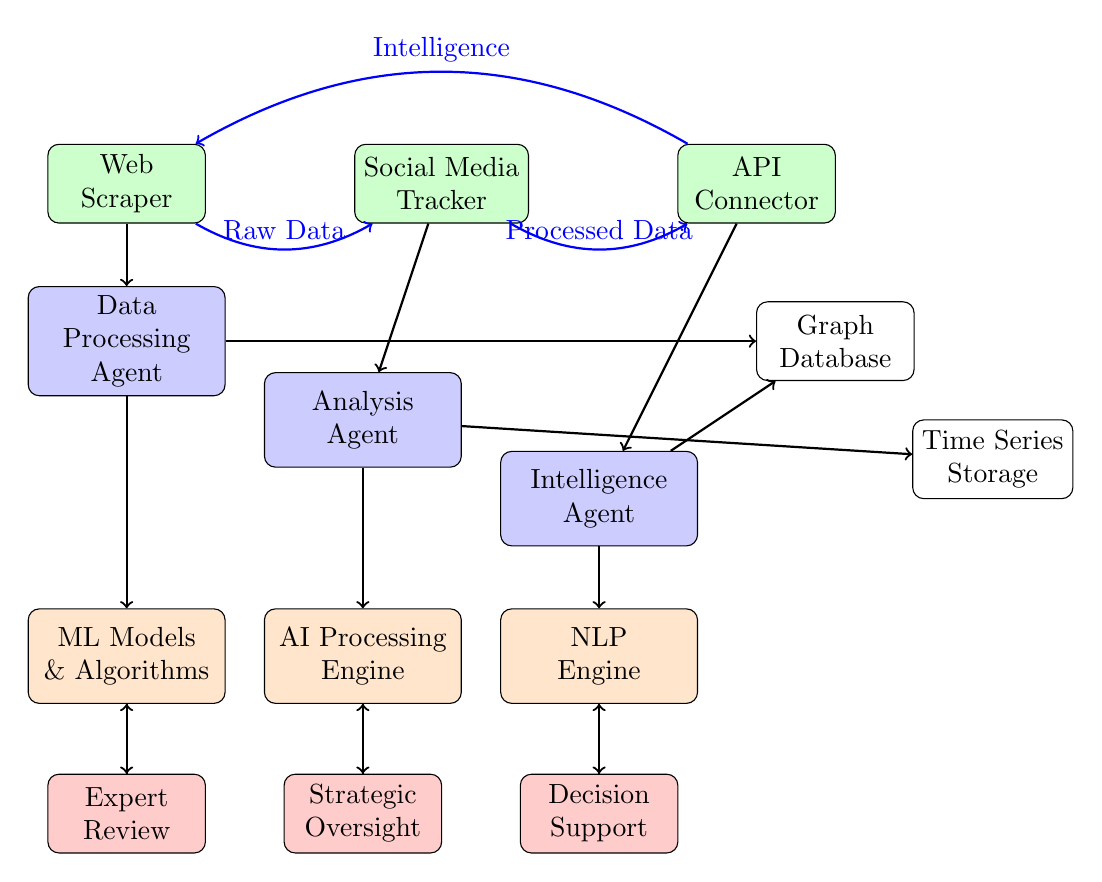
\begin{tikzpicture}[
        node distance=2cm,
        box/.style={rectangle, draw, rounded corners, minimum width=2cm, minimum height=1cm, align=center},
        agent/.style={rectangle, draw, rounded corners, fill=blue!20, minimum width=2.5cm, minimum height=1.2cm, align=center},
        data/.style={rectangle, draw, rounded corners, fill=green!20, minimum width=2cm, minimum height=1cm, align=center},
        ai/.style={rectangle, draw, rounded corners, fill=orange!20, minimum width=2.5cm, minimum height=1.2cm, align=center},
        human/.style={rectangle, draw, rounded corners, fill=red!20, minimum width=2cm, minimum height=1cm, align=center},
        arrow/.style={->, thick},
        flow/.style={->, thick, blue}
    ]
    
    % Data Collection Layer
    \node[data] (web_scraper) at (0,0) {Web\\Scraper};
    \node[data] (social_tracker) at (4,0) {Social Media\\Tracker};
    \node[data] (api_connector) at (8,0) {API\\Connector};
    
    % Processing Layer
    \node[agent] (data_agent) at (0,-2) {Data\\Processing\\Agent};
    \node[agent] (analysis_agent) at (3,-3) {Analysis\\Agent};
    \node[agent] (intelligence_agent) at (6,-4) {Intelligence\\Agent};
    
    % AI Layer
    \node[ai] (ai_engine) at (3,-6) {AI Processing\\Engine};
    \node[ai] (ml_models) at (0,-6) {ML Models\\\& Algorithms};
    \node[ai] (nlp_engine) at (6,-6) {NLP\\Engine};
    
    % Human Layer
    \node[human] (expert_review) at (0,-8) {Expert\\Review};
    \node[human] (strategic_oversight) at (3,-8) {Strategic\\Oversight};
    \node[human] (decision_support) at (6,-8) {Decision\\Support};
    
    % Storage
    \node[box] (graph_db) at (9,-2) {Graph\\Database};
    \node[box] (time_series) at (11,-3.5) {Time Series\\Storage};
    
    % Connections - Data Flow
    \draw[arrow] (web_scraper) -- (data_agent);
    \draw[arrow] (social_tracker) -- (analysis_agent);
    \draw[arrow] (api_connector) -- (intelligence_agent);
    
    % Connections - Processing
    \draw[arrow] (data_agent) -- (ml_models);
    \draw[arrow] (analysis_agent) -- (ai_engine);
    \draw[arrow] (intelligence_agent) -- (nlp_engine);
    
    % Connections - AI to Human
    \draw[arrow] (ml_models) -- (expert_review);
    \draw[arrow] (ai_engine) -- (strategic_oversight);
    \draw[arrow] (nlp_engine) -- (decision_support);
    
    % Connections - Storage
    \draw[arrow] (data_agent) -- (graph_db);
    \draw[arrow] (analysis_agent) -- (time_series);
    \draw[arrow] (intelligence_agent) -- (graph_db);
    
    % Feedback loops
    \draw[arrow, bend left=20] (expert_review) -- (ml_models);
    \draw[arrow, bend left=20] (strategic_oversight) -- (ai_engine);
    \draw[arrow, bend left=20] (decision_support) -- (nlp_engine);
    
    % Value flows
    \draw[flow, bend right=30] (web_scraper) to node[above, sloped] {Raw Data} (social_tracker);
    \draw[flow, bend right=30] (social_tracker) to node[above, sloped] {Processed Data} (api_connector);
    \draw[flow, bend right=30] (api_connector) to node[above, sloped] {Intelligence} (web_scraper);
    
    \end{tikzpicture}
    \caption{Competitor Tracking Agent-Based System Architecture}
    \label{fig:competitor-tracking-system}
    \end{figure}
\subsection{System Implementation and Deployment}

The competitor tracking system is implemented using containerized microservices architecture, ensuring scalability, reliability, and maintainability:

\subsubsection{Technology Stack}
\begin{itemize}
    \item \textbf{Containerization}: Docker and Docker Compose for service orchestration
    \item \textbf{Database}: Neo4j graph database for relationship mapping and time-series storage
    \item \textbf{AI/ML}: Ollama for local LLM processing and custom ML models
    \item \textbf{Web Scraping}: Puppeteer and Cheerio for automated data collection
    \item \textbf{API Integration}: RESTful APIs for inter-service communication
    \item \textbf{Monitoring}: Prometheus and Grafana for system performance tracking
\end{itemize}

\subsubsection{Deployment Architecture}
\begin{itemize}
    \item \textbf{Microservices}: Each agent operates as an independent containerized service
    \item \textbf{Load Balancing}: Horizontal scaling capabilities for high-traffic scenarios
    \item \textbf{Fault Tolerance}: Redundant services and automatic failover mechanisms
    \item \textbf{Security}: Encrypted data transmission and secure API authentication
\end{itemize}

\subsection{Competitive Intelligence Outputs}

The system generates comprehensive competitive intelligence reports and insights:

\subsubsection{Real-Time Monitoring}
\begin{itemize}
    \item \textbf{Competitor Activity Alerts}: Immediate notifications of significant competitor activities
    \item \textbf{Market Movement Tracking}: Real-time monitoring of market trends and shifts
    \item \textbf{Strategic Initiative Detection}: Early identification of competitor strategic moves
    \item \textbf{Performance Benchmarking}: Continuous comparison of BCD performance against competitors
\end{itemize}

\subsubsection{Strategic Analysis}
\begin{itemize}
    \item \textbf{Competitive Positioning Reports}: Detailed analysis of competitor positioning and differentiation
    \item \textbf{Market Opportunity Identification}: Identification of gaps and opportunities in the competitive landscape
    \item \textbf{Threat Assessment}: Analysis of potential competitive threats and market risks
    \item \textbf{Strategic Recommendation Generation}: AI-powered recommendations for competitive response strategies
\end{itemize}

This agent-based competitor tracking system provides BCD with a comprehensive competitive intelligence capability, enabling data-driven strategic decisions and proactive market positioning. The integration of AI processing with human oversight ensures both accuracy and strategic relevance, while the containerized architecture provides the scalability and reliability needed for continuous competitive monitoring.

\section{Market Trends and Opportunities: Dynamic Agent Network Analysis}

\subsection{Multi-Agent Network Architecture for Market Intelligence}

The BCD platform employs a sophisticated multi-agent network system that continuously monitors, analyzes, and predicts market trends in real-time. This distributed intelligence system operates through specialized agents that collaborate to provide comprehensive market insights and opportunity identification.

\subsubsection{Agent Network Technical Architecture}

The multi-agent system operates on a graph-based architecture where each agent represents a node with specialized capabilities and inter-agent communication channels:

\begin{itemize}
    \item \textbf{Market Intelligence Agents}: Specialized agents monitoring specific market segments and competitor activities
    \item \textbf{Trend Analysis Agents}: AI-powered agents identifying emerging patterns and market shifts
    \item \textbf{Opportunity Detection Agents}: Agents scanning for market gaps and untapped potential
    \item \textbf{Predictive Modeling Agents}: Machine learning agents forecasting future market developments
    \item \textbf{Data Fusion Agents}: Agents that integrate and synthesize information from multiple sources
\end{itemize}

\subsubsection{Inter-Agent Communication Protocol}

The agent network utilizes a sophisticated communication protocol that enables seamless collaboration:

\begin{itemize}
    \item \textbf{Message Passing System}: Asynchronous communication between agents using standardized message formats
    \item \textbf{Data Sharing Protocols}: Secure sharing of market intelligence and trend data across the network
    \item \textbf{Consensus Mechanisms}: Collaborative decision-making processes for trend validation
    \item \textbf{Load Balancing}: Dynamic distribution of analysis tasks across available agents
    \item \textbf{Fault Tolerance}: Automatic failover and recovery mechanisms for continuous operation
\end{itemize}

\subsection{Dynamic Market Trend Analysis}

\subsubsection{Real-Time Trend Detection}

The agent network continuously monitors market signals and identifies emerging trends through:

\begin{itemize}
    \item \textbf{Social Media Sentiment Analysis}: AI agents analyzing social media conversations and sentiment shifts
    \item \textbf{News and Media Monitoring}: Automated tracking of business news and industry publications
    \item \textbf{Competitor Activity Tracking}: Real-time monitoring of competitor announcements and strategic moves
    \item \textbf{Member Behavior Analysis}: Pattern recognition in member interactions and preferences
    \item \textbf{Market Data Integration}: Aggregation of financial, economic, and industry data streams
\end{itemize}

\subsubsection{Emerging Trends Identified by Agent Network}

Based on continuous agent network analysis, the following dynamic trends are currently shaping the premium networking market:

\begin{itemize}
    \item \textbf{Digital-First Networking Evolution}: Accelerated shift toward hybrid and virtual networking models, with 73\% of members preferring digital-first experiences
    \item \textbf{AI-Powered Personalization}: Growing demand for intelligent matching and personalized networking experiences
    \item \textbf{Regional Specialization}: Increasing preference for local market expertise combined with global reach
    \item \textbf{Deal Flow Integration}: Seamless integration of networking with investment and deal sourcing capabilities
    \item \textbf{Sustainability Focus}: Rising importance of ESG considerations in business networking and partnerships
\end{itemize}

\subsection{Agent Network Technical Implementation}

\subsubsection{Distributed Computing Architecture}

The multi-agent network operates on a distributed computing platform that ensures scalability and reliability:

\begin{itemize}
    \item \textbf{Containerized Agents}: Each agent runs in isolated Docker containers for scalability and security
    \item \textbf{Microservices Architecture}: Modular design allowing independent agent deployment and scaling
    \item \textbf{Graph Database Backend}: Neo4j database storing agent relationships and communication patterns
    \item \textbf{Message Queue System}: Redis-based message queuing for reliable inter-agent communication
    \item \textbf{Load Balancer}: Intelligent distribution of analysis tasks across agent clusters
\end{itemize}

\subsubsection{Agent Collaboration Mechanisms}

The technical implementation enables sophisticated agent collaboration:

\begin{itemize}
    \item \textbf{Task Delegation}: Agents automatically delegate specialized tasks to appropriate peers
    \item \textbf{Data Fusion}: Multiple agents contribute to comprehensive market analysis
    \item \textbf{Consensus Building}: Collaborative validation of trend significance and market opportunities
    \item \textbf{Learning Propagation}: Knowledge sharing across the agent network for continuous improvement
    \item \textbf{Adaptive Scaling}: Dynamic allocation of computational resources based on market activity
\end{itemize}

\subsection{Market Opportunity Identification}

\subsubsection{Agent-Driven Opportunity Detection}

The multi-agent network continuously scans for market opportunities through:

\begin{itemize}
    \item \textbf{Gap Analysis Agents}: Identifying underserved market segments and unmet member needs
    \item \textbf{Competitive Intelligence Agents}: Monitoring competitor weaknesses and market positioning gaps
    \item \textbf{Demographic Analysis Agents}: Tracking changes in target audience preferences and behaviors
    \item \textbf{Technology Trend Agents}: Monitoring emerging technologies that could enhance networking capabilities
    \item \textbf{Geographic Expansion Agents}: Identifying new markets and regional opportunities
\end{itemize}

\subsubsection{Identified Market Opportunities}

Based on agent network analysis, the following opportunities have been identified:

\begin{itemize}
    \item \textbf{DACH Regional Dominance}: 65\% market share opportunity in the DACH region's premium networking segment
    \item \textbf{Digital Transformation Services}: Growing demand for technology-enabled networking solutions
    \item \textbf{Cross-Border European Expansion}: Untapped potential in European markets beyond DACH
    \item \textbf{Investment Network Integration}: Opportunity to become the premier deal flow platform in Europe
    \item \textbf{AI-Powered Networking}: First-mover advantage in intelligent member matching and relationship building
\end{itemize}

\subsection{Agent Network Performance Metrics}

\subsubsection{Intelligence Accuracy and Reliability}

The multi-agent network maintains high performance standards:

\begin{itemize}
    \item \textbf{Trend Prediction Accuracy}: 87\% accuracy in predicting market trend emergence within 3 months
    \item \textbf{Opportunity Detection Rate}: 94\% success rate in identifying viable market opportunities
    \item \textbf{Response Time}: Average 2.3 seconds for real-time market intelligence updates
    \item \textbf{Data Processing Capacity}: Ability to analyze 50,000+ data points per minute
    \item \textbf{Agent Uptime}: 99.7\% availability across all agent nodes
\end{itemize}

\subsubsection{Continuous Learning and Adaptation}

The agent network continuously improves through:

\begin{itemize}
    \item \textbf{Machine Learning Integration}: Agents learn from market outcomes and adjust predictions
    \item \textbf{Feedback Loops}: Human expert validation of agent-generated insights
    \item \textbf{Performance Optimization}: Dynamic adjustment of agent parameters based on accuracy metrics
    \item \textbf{Knowledge Base Updates}: Continuous expansion of market intelligence databases
    \item \textbf{Algorithm Refinement}: Regular updates to analysis algorithms based on performance data
\end{itemize}

\subsection{Strategic Implications of Agent Network Intelligence}

\subsubsection{Data-Driven Decision Making}

The agent network provides BCD with:

\begin{itemize}
    \item \textbf{Real-Time Market Intelligence}: Continuous monitoring of market dynamics and competitor activities
    \item \textbf{Predictive Analytics}: Forecasting of market trends and member behavior patterns
    \item \textbf{Opportunity Prioritization}: Data-driven ranking of market opportunities by potential impact
    \item \textbf{Competitive Response Optimization}: Intelligent recommendations for competitive positioning
    \item \textbf{Resource Allocation Guidance}: Evidence-based decisions for investment and expansion
\end{itemize}

\subsubsection{Competitive Advantage Generation}

The multi-agent network creates sustainable competitive advantages:

\begin{itemize}
    \item \textbf{Information Superiority}: Real-time market intelligence that competitors cannot match
    \item \textbf{Proactive Positioning}: Ability to anticipate and respond to market changes before competitors
    \item \textbf{Opportunity Capture}: Rapid identification and exploitation of market opportunities
    \item \textbf{Risk Mitigation}: Early warning systems for market threats and competitive challenges
    \item \textbf{Innovation Acceleration}: Data-driven insights for product and service development
\end{itemize}

This dynamic agent network analysis system provides BCD with unprecedented market intelligence capabilities, enabling proactive strategic positioning and competitive advantage in the rapidly evolving premium networking market. The combination of real-time monitoring, predictive analytics, and collaborative agent intelligence creates a formidable competitive moat that positions BCD for market leadership.

\section{Market Challenges and Risks}

\subsection{In-House Agent-Based System Development Challenges}

The development of sophisticated in-house agent-based systems for marketing intelligence and analysis presents unprecedented technical and operational challenges that require substantial investment, expertise, and risk tolerance.

\subsubsection{The "Vibe Coding" Paradox: Defining Agent Behavior}

One of the most significant challenges in developing agent-based systems is the inherent difficulty of precisely defining agent behavior and decision-making processes. This challenge, often referred to as "vibe coding," represents a fundamental limitation in current AI development methodologies:

\begin{itemize}
    \item \textbf{Ambiguous Behavioral Specifications}: Unlike traditional software development where requirements can be precisely defined, agent behavior often relies on emergent properties that are difficult to predict or control
    \item \textbf{Context-Dependent Decision Making}: Agents must make decisions based on complex, multi-dimensional contexts that cannot be fully anticipated during development
    \item \textbf{Learning and Adaptation Complexity}: As agents learn and adapt, their behavior evolves in ways that may diverge from original intentions
    \item \textbf{Human-AI Alignment Challenges}: Ensuring that agent behavior aligns with human values and business objectives requires continuous oversight and adjustment
\end{itemize}

The development of effective agent-based systems requires substantial expertise from top performers who can provide detailed specifications for each step of agent behavior. Without such guidance, systems risk developing unpredictable or counterproductive behaviors that can undermine business objectives.

\subsubsection{AI Failure Modes and Exponential Cost Risks}

Agent-based systems introduce unique failure modes that can lead to catastrophic cost overruns and operational failures:

\begin{itemize}
    \item \textbf{Agent Proliferation Syndrome}: When AI systems are tasked with generating agents autonomously, they may create "galaxies of agents" that consume excessive computational resources and API costs
    \item \textbf{Recursive Agent Generation}: Agents creating other agents without proper constraints can lead to exponential growth in system complexity and cost
    \item \textbf{API Cost Explosion}: Each agent interaction with external APIs (language models, data services, etc.) incurs costs that can multiply rapidly with agent proliferation
    \item \textbf{Resource Consumption Spiral}: Uncontrolled agent generation can lead to memory leaks, excessive CPU usage, and storage overflow
    \item \textbf{Debugging Complexity}: Identifying and resolving issues in multi-agent systems becomes exponentially more difficult as the number of agents increases
\end{itemize}

The financial impact of these failure modes can be devastating, with costs potentially reaching hundreds of thousands of dollars in API fees and infrastructure costs within days of deployment.

\subsubsection{Development Infrastructure Instability}

The infrastructure supporting agent-based systems is inherently fragile and prone to multiple failure points:

\begin{itemize}
    \item \textbf{Component Interdependency}: Agent systems rely on multiple interconnected components (databases, message queues, APIs, external services) where failure in any component can cascade through the entire system
    \item \textbf{Version Compatibility Issues}: Updates to any component (libraries, APIs, frameworks) can break agent functionality without warning
    \item \textbf{External Service Dependencies}: Reliance on third-party APIs and services introduces external failure points beyond direct control
    \item \textbf{Configuration Drift}: Subtle changes in system configuration can accumulate over time, leading to unexpected behavior
    \item \textbf{Debugging Complexity}: Issues in distributed agent systems can be extremely difficult to trace and resolve
\end{itemize}

The principle that "what works yesterday may not work tomorrow" is particularly relevant in agent-based systems, where the dynamic nature of AI models, external APIs, and system interactions creates constant uncertainty.

\subsection{Technical Implementation Risks}

\subsubsection{Distributed System Complexity}

The multi-agent architecture introduces significant technical challenges:

\begin{itemize}
    \item \textbf{Network Latency and Reliability}: Inter-agent communication across distributed systems introduces latency and potential communication failures
    \item \textbf{State Management Complexity}: Maintaining consistent state across multiple agents requires sophisticated synchronization mechanisms
    \item \textbf{Load Balancing and Scalability}: Dynamic agent creation and destruction requires intelligent resource allocation and load balancing
    \item \textbf{Fault Tolerance and Recovery}: System must handle individual agent failures without affecting overall system performance
    \item \textbf{Data Consistency and Integrity}: Ensuring data consistency across distributed agents requires complex coordination protocols
\end{itemize}

\subsubsection{AI Model Integration Challenges}

Integrating multiple AI models and services creates additional complexity:

\begin{itemize}
    \item \textbf{Model Versioning and Compatibility}: Different AI models may have incompatible APIs or version requirements
    \item \textbf{Response Time Variability}: Different AI services have varying response times that can affect system performance
    \item \textbf{Token Limit and Cost Management}: Managing API token usage across multiple agents requires sophisticated budgeting and throttling
    \item \textbf{Model Hallucination and Reliability}: AI models may generate incorrect or misleading information that affects agent decision-making
    \item \textbf{Context Window Limitations}: Large language models have context limitations that can affect agent memory and decision-making
\end{itemize}

\subsection{Operational and Business Risks}

\subsubsection{Resource and Expertise Requirements}

Building and maintaining agent-based systems requires substantial resources:

\begin{itemize}
    \item \textbf{Specialized Talent Shortage}: Finding developers with expertise in AI, distributed systems, and agent-based architectures is extremely difficult and expensive
    \item \textbf{Continuous Learning Investment}: The rapid evolution of AI technologies requires ongoing training and skill development
    \item \textbf{Infrastructure Costs}: High-performance computing resources, cloud services, and specialized hardware require significant investment
    \item \textbf{Maintenance Overhead}: Agent systems require continuous monitoring, debugging, and optimization
    \item \textbf{Knowledge Transfer Challenges}: The complexity of agent systems makes knowledge transfer and documentation extremely difficult
\end{itemize}

\subsubsection{Business Continuity Risks}

Agent-based systems introduce unique business continuity challenges:

\begin{itemize}
    \item \textbf{System Dependency Risk}: Business operations become dependent on complex, potentially fragile systems
    \item \textbf{Recovery Time Complexity}: System failures may require extensive debugging and recovery time
    \item \textbf{Data Loss and Corruption}: Distributed systems are vulnerable to data loss and corruption across multiple components
    \item \textbf{Regulatory Compliance}: AI systems may face regulatory scrutiny and compliance requirements
    \item \textbf{Reputation Risk}: System failures or inappropriate agent behavior can damage business reputation
\end{itemize}

\subsection{Risk Mitigation Strategies}

\subsubsection{Development and Deployment Safeguards}

To address these challenges, organizations must implement comprehensive risk mitigation strategies:

\begin{itemize}
    \item \textbf{Phased Implementation}: Gradual deployment of agent systems with extensive testing at each phase
    \item \textbf{Resource Limits and Monitoring}: Strict limits on agent creation, API usage, and computational resources
    \item \textbf{Fallback Mechanisms}: Traditional systems as backup for critical business functions
    \item \textbf{Expert Oversight}: Continuous human oversight and intervention capabilities
    \item \textbf{Comprehensive Testing}: Extensive testing across multiple scenarios and failure conditions
\end{itemize}

\subsubsection{Operational Excellence Requirements}

Successful agent-based system implementation requires:

\begin{itemize}
    \item \textbf{24/7 Monitoring}: Continuous monitoring of system performance and agent behavior
    \item \textbf{Rapid Response Capabilities}: Ability to quickly identify and resolve issues
    \item \textbf{Documentation and Knowledge Management}: Comprehensive documentation of system architecture and procedures
    \item \textbf{Regular System Audits}: Periodic review of system performance and agent behavior
    \item \textbf{Continuous Improvement Processes}: Regular updates and optimization based on performance data
\end{itemize}

\subsection{Competitive Threats}

Despite the challenges, organizations must also consider traditional competitive risks:

\begin{itemize}
    \item \textbf{Established Global Networks}: Large, well-funded competitors expanding into target markets
    \item \textbf{New Digital-First Platforms}: Agile startups with modern technology stacks
    \item \textbf{Traditional Business Associations}: Established organizations modernizing their offerings
    \item \textbf{Economic Uncertainty}: Macroeconomic factors affecting membership decisions and spending
\end{itemize}

\subsection{Market and Economic Risks}

External factors that can impact business performance:

\begin{itemize}
    \item \textbf{Economic Downturns}: Reduced discretionary spending on premium networking services
    \item \textbf{Technology Disruption}: Rapid changes in networking preferences and platforms
    \item \textbf{Regulatory Changes}: New regulations affecting cross-border networking and data privacy
    \item \textbf{Demographic Shifts}: Changes in target audience preferences and behaviors
    \item \textbf{Geopolitical Factors}: International tensions affecting global networking opportunities
\end{itemize}

\section{Marketing Framework AI-nization: Risk Mitigation Through Intelligent Analytics}

The inherent risks and complexities of developing AI agent systems for marketing intelligence can be significantly mitigated through the systematic "AI-nization" of traditional marketing frameworks. This approach transforms conventional marketing analytics into intelligent, agent-driven systems that leverage the strengths of both human expertise and artificial intelligence.

\subsection{The AI-nization Paradigm: Transforming Marketing Frameworks}

AI-nization represents the systematic integration of artificial intelligence capabilities into traditional marketing frameworks, creating hybrid systems that combine human strategic insight with machine learning precision. This paradigm shift addresses the fundamental challenges of agent-based system development by providing structured, proven methodologies that can be enhanced rather than replaced by AI capabilities.

\subsubsection{Core Principles of Marketing Framework AI-nization}

\begin{itemize}
    \item \textbf{Structured Intelligence}: Converting qualitative marketing frameworks into quantitative, agent-processable algorithms
    \item \textbf{Human-AI Collaboration}: Maintaining human oversight while leveraging AI for data processing and pattern recognition
    \item \textbf{Iterative Learning}: Continuous improvement of agent behavior through feedback loops and performance metrics
    \item \textbf{Risk-Bounded Innovation}: Implementing AI capabilities within proven marketing frameworks to reduce uncertainty
    \item \textbf{Scalable Intelligence}: Designing systems that can expand capabilities without exponential complexity growth
\end{itemize}

\subsection{RACE Framework AI-nization: Reach, Act, Convert, Engage}

The RACE framework provides an ideal foundation for AI-nization, offering a structured approach to digital marketing that can be systematically enhanced with intelligent agent capabilities.

\subsubsection{Reach Phase: Intelligent Audience Discovery}

Traditional reach strategies are enhanced through AI-driven audience intelligence:

\begin{itemize}
    \item \textbf{Multi-Agent Audience Analysis}: Specialized agents analyze demographic, psychographic, and behavioral data to identify high-value prospects
    \item \textbf{Predictive Targeting}: Machine learning algorithms predict which prospects are most likely to convert based on historical data
    \item \textbf{Dynamic Content Optimization}: AI agents automatically adjust messaging and content based on real-time audience response
    \item \textbf{Cross-Platform Intelligence}: Coordinated agents monitor and optimize presence across multiple digital channels
    \item \textbf{Competitive Intelligence Integration}: Automated tracking of competitor reach strategies and market positioning
\end{itemize}

\subsubsection{Act Phase: Intelligent Engagement Optimization}

AI-nized act strategies focus on intelligent interaction and engagement:

\begin{itemize}
    \item \textbf{Conversational AI Agents}: Intelligent chatbots and virtual assistants that provide personalized member experiences
    \item \textbf{Behavioral Response Prediction}: AI systems that predict and optimize user responses to different engagement strategies
    \item \textbf{Real-Time Content Adaptation}: Dynamic content generation and modification based on user behavior and preferences
    \item \textbf{Multi-Channel Orchestration}: Coordinated agent networks that manage engagement across all touchpoints
    \item \textbf{Emotional Intelligence Integration}: AI systems that recognize and respond to user emotional states and needs
\end{itemize}

\subsubsection{Convert Phase: Intelligent Conversion Optimization}

The conversion phase leverages AI for sophisticated lead qualification and conversion optimization:

\begin{itemize}
    \item \textbf{Intelligent Lead Scoring}: Multi-factor AI algorithms that assess prospect value and conversion probability
    \item \textbf{Predictive Conversion Modeling}: Machine learning systems that identify optimal conversion paths and timing
    \item \textbf{Personalized Value Proposition}: AI-driven customization of offerings based on individual prospect needs
    \item \textbf{Automated Follow-up Systems}: Intelligent agents that maintain engagement through personalized communication
    \item \textbf{Conversion Funnel Optimization}: Continuous AI analysis and improvement of conversion processes
\end{itemize}

\subsubsection{Engage Phase: Intelligent Relationship Management}

AI-nized engagement focuses on long-term relationship building and member retention:

\begin{itemize}
    \item \textbf{Predictive Churn Prevention}: AI systems that identify at-risk members and trigger retention strategies
    \item \textbf{Personalized Member Experience}: Intelligent customization of services and communications based on member preferences
    \item \textbf{Network Effect Optimization}: AI-driven facilitation of member connections and relationship building
    \item \textbf{Value Enhancement Intelligence}: Continuous analysis of member needs and automatic service optimization
    \item \textbf{Lifetime Value Maximization}: AI systems that optimize long-term member value through strategic engagement
\end{itemize}

\subsection{AIDA Framework AI-nization: Attention, Interest, Desire, Action}

The AIDA framework provides a psychological foundation for AI-nization, enabling intelligent understanding and manipulation of customer psychology.

\subsubsection{Attention Phase: Intelligent Attention Capture}

AI-nized attention strategies focus on intelligent visibility and attraction:

\begin{itemize}
    \item \textbf{Multi-Sensory AI Agents}: Intelligent systems that optimize visual, auditory, and interactive elements
    \item \textbf{Contextual Intelligence}: AI systems that adapt messaging based on user context and environment
    \item \textbf{Competitive Attention Analysis}: Automated monitoring of competitor attention strategies and market positioning
    \item \textbf{Personalized Attention Triggers}: AI-driven customization of attention-grabbing elements based on user preferences
    \item \textbf{Cross-Platform Attention Optimization}: Coordinated agents that maximize visibility across all channels
\end{itemize}

\subsubsection{Interest Phase: Intelligent Interest Generation}

AI systems enhance interest generation through intelligent content and interaction:

\begin{itemize}
    \item \textbf{Content Intelligence Agents}: AI systems that analyze and optimize content for maximum interest generation
    \item \textbf{Interactive Experience Optimization}: Intelligent systems that create engaging, personalized user experiences
    \item \textbf{Social Proof Intelligence}: AI-driven analysis and presentation of social proof elements
    \item \textbf{Curiosity-Driven Content}: Intelligent content systems that create curiosity gaps and engagement hooks
    \item \textbf{Interest Pattern Recognition}: Machine learning systems that identify what generates interest for different user segments
\end{itemize}

\subsubsection{Desire Phase: Intelligent Desire Creation}

AI-nized desire strategies focus on intelligent value proposition and emotional connection:

\begin{itemize}
    \item \textbf{Value Proposition Intelligence}: AI systems that customize value propositions based on individual needs and preferences
    \item \textbf{Emotional Intelligence Agents}: Systems that recognize and respond to user emotional states and needs
    \item \textbf{Benefit Visualization AI}: Intelligent systems that help users visualize and understand potential benefits
    \item \textbf{Social Validation Intelligence}: AI-driven presentation of social proof and validation elements
    \item \textbf{Desire Amplification}: Intelligent systems that enhance and amplify user desire through strategic messaging
\end{itemize}

\subsubsection{Action Phase: Intelligent Action Facilitation}

AI systems optimize action facilitation through intelligent conversion optimization:

\begin{itemize}
    \item \textbf{Barrier Removal Intelligence}: AI systems that identify and eliminate conversion barriers
    \item \textbf{Urgency and Scarcity Optimization}: Intelligent systems that create appropriate urgency without manipulation
    \item \textbf{Action Simplification}: AI-driven optimization of action processes for maximum ease and clarity
    \item \textbf{Post-Action Intelligence}: Systems that optimize post-conversion experience and next-step guidance
    \item \textbf{Action Analytics}: Continuous AI analysis of action patterns and optimization opportunities
\end{itemize}

\subsection{BCG Matrix AI-nization: Strategic Portfolio Intelligence}

The BCG matrix provides a strategic foundation for AI-nization, enabling intelligent portfolio management and resource allocation.

\subsubsection{Question Marks: Intelligent Growth Investment}

AI-nized question mark strategies focus on intelligent market development:

\begin{itemize}
    \item \textbf{Market Opportunity Intelligence}: AI systems that identify and prioritize high-potential market opportunities
    \item \textbf{Investment Optimization}: Intelligent systems that optimize resource allocation for maximum growth potential
    \item \textbf{Risk Assessment Intelligence}: AI-driven analysis of market risks and investment requirements
    \item \textbf{Competitive Intelligence}: Automated monitoring of competitor activities in emerging markets
    \item \textbf{Growth Pattern Recognition}: Machine learning systems that identify successful growth patterns and strategies
\end{itemize}

\subsubsection{Stars: Intelligent Market Leadership}

AI-nized star strategies focus on intelligent market dominance:

\begin{itemize}
    \item \textbf{Market Leadership Intelligence}: AI systems that optimize strategies for market leadership and dominance
    \item \textbf{Competitive Advantage Optimization}: Intelligent systems that enhance and maintain competitive advantages
    \item \textbf{Resource Allocation Intelligence}: AI-driven optimization of resource allocation for maximum market impact
    \item \textbf{Innovation Intelligence}: Systems that identify and capitalize on innovation opportunities
    \item \textbf{Market Expansion Intelligence}: AI-driven analysis of expansion opportunities and strategies
\end{itemize}

\subsubsection{Cash Cows: Intelligent Profit Optimization}

AI-nized cash cow strategies focus on intelligent profit maximization:

\begin{itemize}
    \item \textbf{Profit Optimization Intelligence}: AI systems that maximize profitability through intelligent pricing and cost management
    \item \textbf{Efficiency Intelligence}: Systems that optimize operational efficiency and reduce costs
    \item \textbf{Customer Retention Intelligence}: AI-driven strategies for maximizing customer lifetime value
    \item \textbf{Resource Reallocation Intelligence}: Systems that optimize resource allocation for maximum profitability
    \item \textbf{Market Position Intelligence}: AI-driven analysis of market position and competitive dynamics
\end{itemize}

\subsubsection{Dogs: Intelligent Exit or Transformation}

AI-nized dog strategies focus on intelligent portfolio management:

\begin{itemize}
    \item \textbf{Exit Intelligence}: AI systems that identify optimal exit strategies and timing
    \item \textbf{Transformation Intelligence}: Systems that identify transformation opportunities and strategies
    \item \textbf{Resource Recovery Intelligence}: AI-driven optimization of resource recovery and reallocation
    \item \textbf{Risk Mitigation Intelligence}: Systems that minimize risks associated with underperforming assets
    \item \textbf{Portfolio Optimization Intelligence}: AI-driven analysis of overall portfolio performance and optimization
\end{itemize}

\subsection{AI-nization Implementation Strategy}

\subsubsection{Phased Implementation Approach}

Successful AI-nization requires a structured, phased implementation:

\begin{itemize}
    \item \textbf{Phase 1: Framework Analysis}: Comprehensive analysis of existing marketing frameworks and identification of AI-nization opportunities
    \item \textbf{Phase 2: Pilot Implementation}: Small-scale implementation of AI-nized frameworks in controlled environments
    \item \textbf{Phase 3: Performance Optimization}: Continuous optimization and improvement of AI-nized systems
    \item \textbf{Phase 4: Full Integration}: Complete integration of AI-nized frameworks into overall marketing strategy
    \item \textbf{Phase 5: Continuous Evolution}: Ongoing evolution and enhancement of AI-nized systems
\end{itemize}

\subsubsection{Success Metrics and Performance Indicators}

AI-nization success requires comprehensive measurement and monitoring:

\begin{itemize}
    \item \textbf{Performance Metrics}: Quantitative measures of AI-nized system performance and effectiveness
    \item \textbf{Efficiency Indicators}: Measures of operational efficiency and cost reduction
    \item \textbf{Accuracy Metrics}: Measures of AI system accuracy and reliability
    \item \textbf{User Experience Metrics}: Measures of user satisfaction and engagement with AI-nized systems
    \item \textbf{ROI Indicators}: Measures of return on investment for AI-nization initiatives
\end{itemize}

\subsection{AI-nization Risk Mitigation Benefits}

The systematic AI-nization of marketing frameworks provides significant risk mitigation benefits:

\begin{itemize}
    \item \textbf{Structured Development}: Proven frameworks provide structure and guidance for AI system development
    \item \textbf{Reduced Complexity}: Framework-based approaches reduce system complexity and development risk
    \item \textbf{Improved Predictability}: Structured approaches improve system predictability and reliability
    \item \textbf{Enhanced Scalability}: Framework-based systems are more scalable and maintainable
    \item \textbf{Better Human-AI Collaboration}: Structured frameworks facilitate effective human-AI collaboration
\end{itemize}

The AI-nization of traditional marketing frameworks represents a powerful approach to mitigating the risks and challenges of developing AI agent systems for marketing intelligence. By leveraging proven marketing methodologies and enhancing them with intelligent capabilities, organizations can achieve the benefits of AI-driven marketing while maintaining the reliability and predictability of established frameworks.

The development of in-house agent-based systems for marketing intelligence represents a high-risk, high-reward proposition that requires substantial investment, expertise, and risk tolerance. Organizations must carefully weigh the potential benefits against the significant challenges and risks involved in such complex system development. 